% Keep these two lines in order to get typesetting to work w/ the funny fonts.
%!TEX TS-program = xelatex
%!TEX encoding = UTF-8 Unicode

\documentclass[12pt]{article}
\usepackage{geometry} % See geometry.pdf for lots of layout options. 
\usepackage[config, font=small, labelfont={sf,bf}, textfont=sf]{caption,subfig}
\usepackage{graphicx}
\usepackage{amssymb}

\usepackage{fontspec,xltxtra,xunicode}
\defaultfontfeatures{Mapping=tex-text}
\setromanfont[Mapping=tex-text]{Fanwood Text}
\setsansfont[Scale=MatchLowercase,Mapping=tex-text]{Gill Sans}
\setmonofont[Scale=MatchLowercase]{Andale Mono}

\title{How People Design for Laser Cutters}
\author{Gabe Johnson}
%\date{} % Activate to display a given date or no date

\begin{document}
\maketitle

\section{Physical Hacking}

There is a growing community of self-described \textit{makers} who
design and build many kinds of physical
things~\cite{gershenfeld-fab}. Some are electronic or robotic gizmos,
while others are composed of traditional material but designed or made
with modern technology. The ranks of these ``new
makers''~\cite{gross-new-makers} include mechanical engineers,
industrial designers, artists, computer programmers, architects, and
many others. It is common for these people to be relatively untrained
in aspects of their craft, such as using modeling software, desiging
or assembling electronics, or making visually appealing physical
constructions. It is rare to find any individual person that is an
expert in all of these topics, but it is common that a person knows
something about a lot of them.

It is possible that we are beginning to see a shift from an economy
based on mass-production (in factories) to one that includes
mass-customization (in homes and community centers). Rapid fabrication
machines continue to decline in price while improving in quality. It
is conceivable that in the not-so-distant future, small manufacturing
machines will be as common as desktop printers~\cite{economist-fab}. A
new sector of small businesses use rapid fabrication to cater to the
needs of hobbyist designers as well as people that need highly
customized goods (e.g. prosthetic limbs)~\cite{nyt-rapidfab}.

The surge of home manufacturing is made possible by a number of
related factors. First, there is a trend away from a culture of
consumption towards a culture of production. This is most visibly
reflected in the democratization of modern media where the users
become the dominant producers of content (e.g. social networking
systems like Facebook or the game Minecraft). People are once again
beginning to participate in the design of the world around them.

Second, there is a developing support structure for the new makers,
including physical shared space, Internet resources, magazines, and
conferences. \textit{Hacker spaces} are physical locations where
people can meet, share ideas, and work on projects. Hacker spaces
commonly have various tools and supplies available to members. Online
stores such as Sparkfun and model sharing sites like Thingiverse and
3D Warehouse give hackers easy access to supplies. There are several
Internet-based companies (e.g. Pokono) that offer fabrication
services. O'Reilly's \textit{Make Magazine} is a popular periodical
catering to this community. O'Reilly also puts on several
\textit{Maker Faire} gatherings every year where physical hackers can
meet.

Last, physical hacking is made accessible by the increasing
availability and affordability of rapid fabrication machines like 3D
printers, CNC mills, and laser cutters. This work focuses on projects
that use laser cutters. Figure~\ref{fig:prices} shows prices for a
comparable~25-Watt,~16''x12'' laser cutter model from Universal Laser
Systems (these values were found on hobbyist web forums). While these
data may not be exact, they do show the price of desktop laser cutting
machines has been cut by almost half in the past ten years. While
still out of reach for most people to afford, they are becoming
inexpensive enough for schools and hacker spaces to own.

% Price information: 
% 2001: 12,900 (ULS 25 watt)
% 2006: 9,995 (ULS 25 watt)
% 2010: 8,500 (ULS 25 watt)
% 2011: 6,850 (ULS 25 watt)
%
%   http://www.rcgroups.com/forums/showthread.php?t=16912 claims that
%   a 25-watt model from Universal Laser systems cost $12,900. Several
%   comments in that thread are in line with that price estimate for
%   home-garage-lab use.
%   http://www.microgeo-usa.com/ProductDetails.asp?ProductCode=universal-laser-VLS2.30
%   currently prices the ULS 25 watt 16x12 unit as costing $6,850.

% http://55-website.com/xo1/ulsinc/english/PDFs/EJ_VL_Article_Reprint.pdf is a press article from 2006 that prices the 25 watt laser at 10,000
\begin{figure}[h] %  figure placement: here, top, bottom, or page
   \centering
   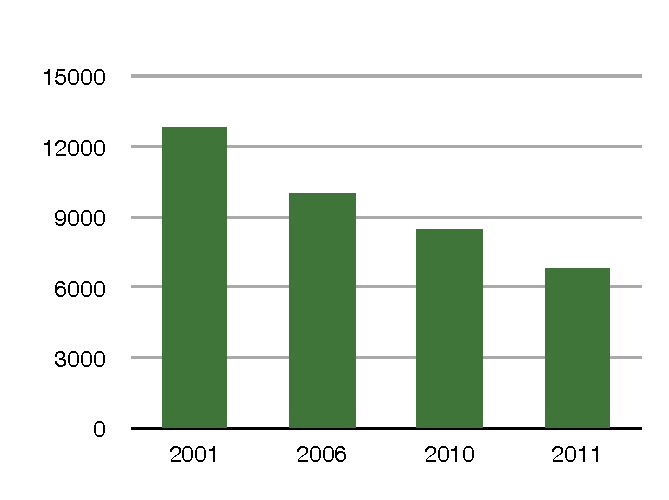
\includegraphics[width=3in]{img/prices.pdf} 
   \caption{Declining prices of Universal Laser Systems 25-Watt 16x12
     inch laser cutter (US Dollars).}
   \label{fig:prices}
\end{figure}

\section{Current Design Practices for Laser Cutting}

\begin{figure}[h] %  figure placement: here, top, bottom, or page
   \centering
   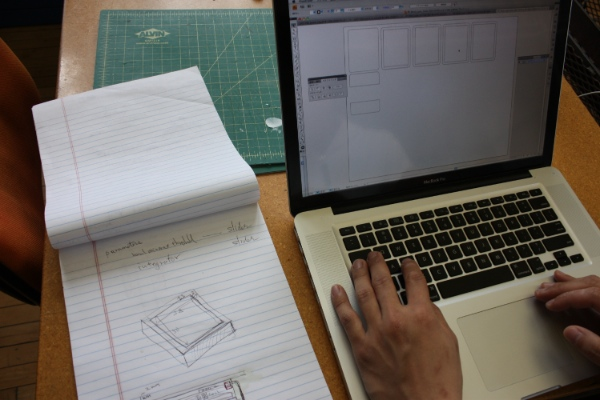
\includegraphics[width=4in]{img/translate-sketch-to-computer.jpg} 
   \caption{A common part of designing for laser cutters: translating
     a hand-made sketch to a computer modeling tool. The sketch
     includes a 3D depiction of the result, with important dimension
     values written down.}
   \label{fig:translating-to-computer}
\end{figure}

Laser cutters (and other rapid fabrication machines) are a relatively
new addition to the design studio. Further, many of the people using
laser cutters are avocational designers that lack formal design
education.

I am currently conducting interviews and observations to better
understand how people think about, model, and make things using laser
cutters. In addition to these interviews I have several years of
exposure and some direct experience on this topic.

\subsection{Laser Cutters and Laser Cut Items}

A laser cutter can be thought of as a very fast, strong, and precise
automated razor blade. They cut through flat material (paper, wood,
plastic, metal, etc.) from directly above.

Some items can be made entirely with a laser cutter. These projects do
not involve other machines or material, aside from the occasional
screw or glue. Other projects might be made partly with a laser
cutter, and partly with other machines. Sometimes an artifact is
designed with to allow it to interact with another object that already
exists. This places additional constraints on the design because it
must conform to existing measurements. The car-mounted smart phone
holder in Figure~\ref{fig:phone-holder} is one such example. If we are
given another similar device with slightly different dimensions, we
might simply change some parameters and cut another holder.

\begin{figure}[h] %  figure placement: here, top, bottom, or page
   \centering
   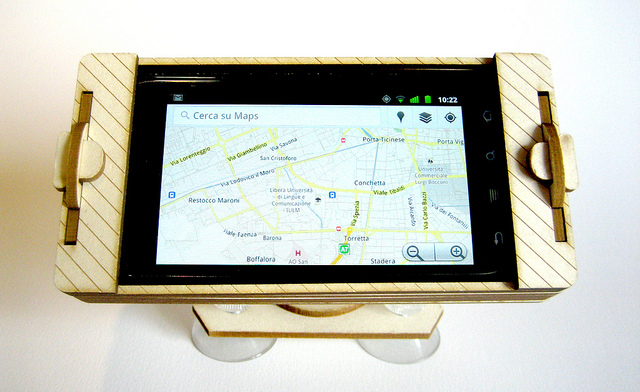
\includegraphics[width=4in]{img/phone-holder.jpg} 
   \caption{A laser-cut smart phone holder designed to fit around a
     particular device and mounted on the dash of a car (by Davide
     Prato).}
   \label{fig:phone-holder}
\end{figure}

\subsection{Current Tools, Current Problems}

Rapid fabrication hardware requires software. Currently, modeling
tools for rapid fabrication are almost exclusively designed for
professional, expert users. The personal computing industry was only
able to take off when intuitive interfaces were developed that allowed
ordinary people to use them. If rapid fabrication is to become common,
software modeling tools must be made accessible by ordinary
users~\cite{lipson-homefactory}.

Today, designers can choose among several modeling tools for laser
cutter projects. As a minimum requirement, the tool must be able to
produce a vector graphics file, where colors indicate which action the
laser takes (e.g. cut through material or etch into it). Adobe
Illustrator is the most commonly used package. Others include Rhino,
InkScape, AutoCAD, and SolidWorks.

Illustrator is a general-purpose vector graphics tool. Specialized
design tools like Rhino or SolidWorks are perhaps more appropriate for
this kind of modeling, but many people are already familiar with
Illustrator from other 2D vector graphics editors. 

I interviewed designers to find out more about their work practices
and better understand how they use their tools. They have
substantially different backgrounds: all have training in some form of
design, ranging from mechanical engineering to graphic design to
architecture. I began by asking each person to describe how they
work. Each designer was able to show me sketches or videos of their
work. While there are subtle (and some substantial) differences in
their processes, each followed the following pattern.

They begin by thinking about a problem and making drawings by
hand. Some sketches are made to think about how to frame the project
(what is it for), while others help reason about how to make it (how
it works, how it fits together). Some designers explicitly noted that
sketching is a necessary part of the process; it would not be possible
to move forward without making freehand drawings. When the idea is
reasonably well-formed they will implement the model with a software
tool. It is common for this to involve translating a hand-made sketch
to a computer model (Figure~\ref{fig:translating-to-computer}). 

Following the interview about their work practices, I gave
participants a sketch (Figure~\ref{fig:interview-sketch}) and asked
them the implement it using their software tool of choice. The purpose
of this task was to learn what problems people met when executing the
common task of translating a sketch to a computer model.

\begin{figure}[h]
\centering 
\subfloat[The part users set out to replicate.] {
  \label{fig:interview-sketch-1} 
  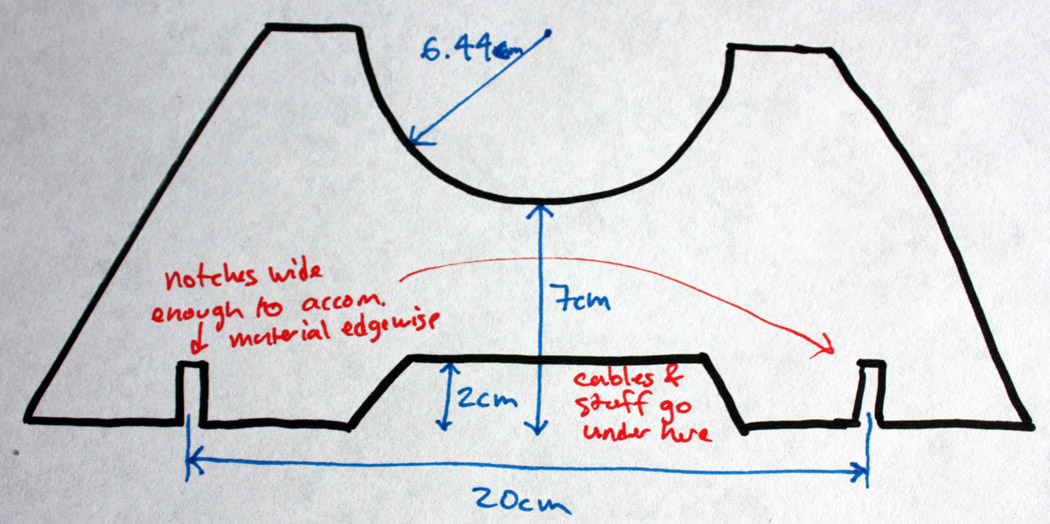
\includegraphics[width=0.5\linewidth]{img/laser-me-1.jpg}
}
\hspace{1cm} \subfloat[Drawing of how the part is used in context.] {
    \label{fig:interview-sketch-2}
    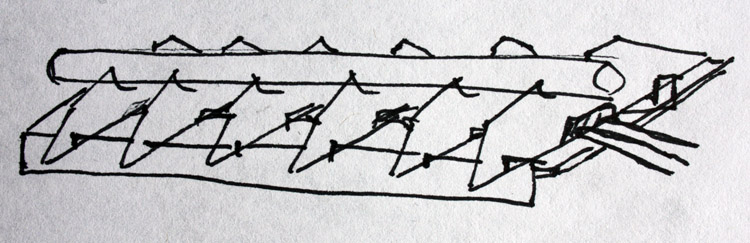
\includegraphics[width=0.5\linewidth]{img/laser-me-2.jpg}
}
\caption{Sketches given to participants to implement in modeling software.}
\label{fig:interview-sketch}
\end{figure}

To design an object suitable for laser cutting, participants used
Illustrator (3 users) or Rhino (1 user). In all cases, a designer's
strategy involved a number of common activities: creating or editing
boundaries, aligning or snapping items, using guide lines or reference
points, measuring distances, specifying or changing lengths and
angles, and creating finished ``cut files'' to send to the laser
cutter. These tasks are in addition to selecting/deselecting, zooming,
panning, and so on.

Participants in this experiment spent a good deal of time on operating
overhead. Overhead includes (1) trying to find the appropriate tool
for the next task, and (2) recovering from errors made when the wrong
tool was selected, or (3) when the tool did not behave consistently
with the user's intention. I have not performed an analysis of the
low-level actions people performed, however I estimate that in my
experiments, more than 50\% of a designers time is spent this way.

For example, one user was aware of Illustrator's ``Path Finder'' tool
and wanted to use it. This user searched the program's menu structure
and hovered over buttons to read tool tips before finding it. Next,
the designer invoked various functions of the Path Finder, using the
keyboard shortcut to undo after each attempt, as he searched for the
correct mode within the Path Finder's subcommand palette. This process
lasted approximately 80 seconds before finally being able to continue.

Participants used the Undo function routinely. The dominant use of
this was to revert after making a single failed attempt to edit some
element. There were a few instances where the designer believed their
current approach was flawed in such a way that it would be better to
back up several dozen operations because a single decision early on
was now observed to be problematic. This is consistent with the study
by Akers \textit{et. al} on the use of undo~\cite{akers-undo}.

One may argue that the problems associated with operating overhead can
be solved by experience or by addressing particular usability
problems. Obviously, masterful Illustrator or Rhino users exist and
would have no problem executing the design task from my
experiment. However, the target audience for this research is
avocational users, not experts. Cooper argues that the set of people
that are truly expert users is not only quite small, it also changes
over time \cite{cooper-inmates}. A person might maintain expert status
for some time, but eventually stops using the program as often, and
eventually becomes an intermediate user, and will generally remain an
intermediate user.

This notion of \textit{perpetual intermediates} is evident in the
designers I interviewed. One participant was a trained graphic
designer (according to the user's peers) was an Illustrator
expert. However, this designer used some rather strange strategies
during the translation task. In order to remove an unwanted line, this
designer chose to create an opaque white rectangle to obscure it,
rather than erase it. (``Don't tell anyone I did this'', he said at
the time).

Similar episodes are common: a person \textit{should} know the
`correct' action, but takes an alternate approach. The alternate way
may achieve the intended effect, but it might be less efficient (more
operations, longer execution time) or it might introduce unwanted
complexity (e.g. invisible white objects in the model).

\section{Implications for Design}

The design observations described above account for a relatively small
slice of hackers designing for laser cutters. It would be unwise to
base an entire research agenda on these few interviews. However, the
current proposal is based on much more than these observations. I have
several years of experience working in an environment where both
undergraduate and graduate students made things with rapid fabrication
machines (including a laser cutter). The recently conducted interviews
validate the observations I have been making for years: current design
tools are hard to learn, provide poor interaction for novice or
occasional users, and do not support idea exploration or informal
representation that is so important during early design.

HCI practitioners often conduct usability studies to uncover
particular problems in applications. The issues uncovered by these
studies are then addressed by changing the software. This iterative
process continues over years, leading to incremental
improvements~\cite{buxton-sketching}.

The interviews and observations from my study confirm that using
current tools involve a great deal of needless overhead for the target
population. However, rather than use this as a basis for incremental
improvement to existing tools, I am interested in developing new tools
the explore an alternate interaction paradigm that is easier and more
effective for typical non-expert designers.

The ultimate goal of any laser cutter project is to make a final
assembly that is made from laser-cut parts. Based on my interviews
with the designers and my own experience, I identify four supporting
goals that serve the larger practical goal of making finished
laser-cut assemblies. These sub-goals include making rough drawings
used to help structure the problem and possible solutions; adding
precise details to drawings; and supporting quick manufacturing and
editing.

\subsection{Supporting Goal 1: Make Rough Representation} 

Designers need strategies to help think about (1) what the whole
assembly should work and look like, (2) what individual pieces should
be made, and (3) how those individual pieces fit together. This is
most commonly done via sketching on paper. Some designers make
rough physical models as well.

Current tools do not make any significant allowance for this goal. The
system proposed here is based on sketching as the primary input
method. This will let users be as rough, abstract, and imprecise as
they like.

\subsection{Supporting Goal 2: Make Precise Specification}

Users would like to be able to easily specify some (but not
necessarily all) dimensions. This is the main purpose of most current
modeling tools, though it is often difficult for people to do it
effectively. For example, in the translate task, there are two notches
that are specified to be 20cm apart. Several participants created
temporary geometry (rectangles and lines) that were set to 20cm long
and placed onscreen. This served as a ruler that the designer could
then use to position the notches. The ruler was then erased.

The proposed tool is somewhat unique in the area of sketch-based
design tools in that it will give users the ability to be quite
precise in identifying dimensions and constraints. It is hoped that
using sketch recognition can allow people to state their intentions
substantially faster than using difficult-to-use structured tools.

\subsection{Supporting Goal 3: Rapid Editing and Manufacture}

Participants reported they use a rapid \textit{model-make-evaluate}
loop. They make several versions of objects with the laser cutter
before it becomes final, because it is important to be able hold it in
their hands. This is sometimes to determine if they made an execution
error. Equally as as often, the physical ``rough draft'' is necessary
to evaluate their idea. Laser cutter projects tend to be fairly quick
and inexpensive in comparison to some other fabrication machinery like
3D printing.

Current tools impose clumsy requirements on designers to prepare
models for laser cutting. For example, the cut line color need to have
the RGB tuple $(0,0,255)$, and line thickness has to be ``hair line''
at 0.01mm. Managing this overhead is time-consuming. The proposed tool
will handle this overhead on the user's behalf.

A common problem exposed by making a physical draft is the discovery
that pieces do not fit together properly. Some dimensions (such as
notch widths) must then change. However, changing one dimension might
have unwanted side-effects, causing a cascade of issues the designer
must identify and fix, while trying to avoid introducing new problems.

The proposed modeling tool assumes that the user might change the
shape or parameterization of models later on, and facilitate these
changes without creating more problems along the way. 

\bibliographystyle{plain}
\addcontentsline{toc}{section}{References}
\bibliography{sketch-bibliography}

\end{document}  
